\documentclass[UTF8,a4paper,11pt,fontset=windows]{ctexart}
\usepackage{amsmath,amssymb,amsthm,bm,booktabs,graphicx,url}
\usepackage[hidelinks]{hyperref}
\graphicspath{{../figures/}}
\setlength{\emergencystretch}{1em}
\newtheorem{proposition}{命题}
\newtheorem{corollary}{推论}
\newcommand{\R}{\mathbb{R}}
\newcommand{\Sstate}{\mathbf{S}}
\newcommand{\vect}{\operatorname{vec}}

\title{面向流式点云识别的固定状态可加 FWP 网络}
\author{Dian Yu\\
University of New South Wales, Sydney, NSW 2052, Australia\\
\texttt{dian.yu2@student.unsw.edu.au}\\
ORCID：\url{https://orcid.org/0009-0002-0107-1014}}
\date{中文正文校对稿}

\begin{document}
\maketitle

\begin{abstract}
多数点云网络通过重新访问已保存的点、重建邻域或执行全局最大池化来获得上下文。这些操作适合离线处理，却使持续增长的点流依赖完整历史。PointProgrammerNet 用三个固定的 $128\times170$ 矩阵取代点历史。每个观测点产生一个表示“写到哪里”的归一化空间地址，以及一个表示“写入什么”的值向量；二者的外积直接加到矩阵中。因此，不同时间或不同设备编码的点云分块可以通过矩阵加法精确合并，状态也支持相减和指数衰减。分割任务在指定坐标读取矩阵，分类任务则在删除全部输入点后仅使用矩阵。本文证明输入顺序不变性、分块与分布式编码等价性、固定保留内存，以及输出对新增证据的连续依赖。使用 XYZ 输入时，模型在 ShapeNetPart 上取得 $92.95\%$ 点准确率、$82.58\%$ 实例 mIoU 和 $79.10\%$ 类别 mIoU，在 ModelNet40 上取得 $86.59\%$ 分类准确率。三个 float32 状态始终占用 255 KiB，与点流长度无关。当累计点数达到 8,192 时，只更新新分块比重建完整状态快 $6.06\times$，相对状态误差仍低于 $10^{-6}$。这些结果展示了用有界、可直接更新和合并的状态取代不断增长的点历史时，其精度代价和实际收益。
\end{abstract}

\noindent\textbf{关键词：}点云；流式学习；可加状态；快速权重程序器；分割；分类

\section{引言}

点云在数学上是无序集合，但传感器通常按时间持续获得点。同一帧内的处理应与点的排列顺序无关，跨帧处理也不应要求重放全部历史。PointNet~\cite{qi2017pointnet} 通过对逐点特征进行对称最大池化获得全局描述，PointNet++~\cite{qi2017pointnetplusplus} 则建立多尺度度量邻域。二者在离线任务中都很有效，但最大值不是可加状态：固定摘要通常无法仅凭简单加法同时支持删除、独立分块合并和连续加权证据。

本文研究一个更严格的设定：一个点写入状态后即可被删除。之后的计算只能访问固定矩阵；分割任务额外允许访问查询坐标。学习得到的键把每个点分配到状态的多个行，二阶值则记录质量、位置、学习内容和交叉矩。所有逐点写入相加后形成固定尺寸状态。

因此，独立点云分块可以直接合并，已保存的子集状态可以相减，旧证据可以衰减，新增点也不需要触碰历史观测。相同代数还可用于分布式感知：边缘设备分别编码不同空间区域或时间片，只传输固定矩阵，中心节点相加后再执行分类或分割。分割头读取一个由坐标查询的连续场，不保存历史点特征；分类头只读取状态行，完整点列表可被删除。

本文的主要贡献如下：
\begin{itemize}
\item 提出三尺度二阶快速权重程序器（FWP）状态，其存储量不随已观测点数增长；
\item 采用可加逐点写入，在不重放分块内容的情况下支持精确流式更新、分层合并和分布式聚合；
\item 设计坐标条件分割头和纯状态分类头，两者都不对解码后的点执行池化；
\item 从理论和实验两方面验证可加性、状态操作、识别精度和更新开销。
\end{itemize}
本文使用的紧凑 PointNet++ 实现是受控基线，用来衡量固定状态约束的精度代价，不声称是标准实现的完整复现。

\section{相关工作}

PointNet 对逐点变换后的特征执行最大池化~\cite{qi2017pointnet}，PointNet++ 进一步引入分层度量邻域~\cite{qi2017pointnetplusplus}。Deep Sets 研究基于求和的置换不变函数~\cite{zaheer2017deepsets}，Set Transformer 使用注意力和诱导点~\cite{lee2019settransformer}。核化注意力可以递归计算~\cite{katharopoulos2020transformers}，快速权重程序器则用可加外积或 delta 修正规则更新记忆~\cite{schlag2021linear}。PointProgrammerNet 将这一思想用于几何数据：固定状态保存空间统计量、学习特征及其二阶关系，并且在释放输入点后仍可使用。本文在 ModelNet40~\cite{wu20153dshapenets} 上测试分类，在由 ShapeNet~\cite{chang2015shapenet} 派生的 ShapeNetPart~\cite{yi2016scalable} 上测试部件分割。

\section{方法}

令点云为 $X=\{\bm{x}_i\}_{i=1}^N$，归一化坐标 $\bm{x}_i\in\R^3$。论文主实验只使用 XYZ。若以后加入法线、颜色或强度，可将它们扩展到写入值中，而不改变状态更新规则。

核心思路是把每个点变成两个向量：空间地址 $\bm k_s(\bm x_i)$ 决定该点分别写入矩阵的哪些行以及写入多少，值 $\bm v_s(\bm x_i)$ 表示需要保存的信息。两个向量的外积是一个矩阵，所有点的外积矩阵相加就是最终状态。因此，对任意两个点多重集合 $A$ 和 $B$，
\begin{equation}
\Sstate(A\uplus B)=\Sstate(A)+\Sstate(B).
\label{eq:add}
\end{equation}
其中，$\uplus$ 表示保留重复点的集合并，$\Sstate(\cdot)$ 表示三个状态矩阵组成的整体。式~\eqref{eq:add} 表明，$A$ 和 $B$ 可以在不同时间甚至不同设备上独立编码，合并时只需矩阵相加，不必再次访问原始点。

模型包含细、中、粗三个分支，记为 $s\in\{f,m,b\}$。三个分支具有完全相同的容量和计算结构：每个状态都是 $R=128$ 行、$D=170$ 列，分割读出网络的尺寸也相同；但三个分支的参数彼此独立。它们的半径初始值分别为 $0.08,0.20,0.60$，随后均可学习。“细、中、粗”只描述初始空间范围，并不人为规定每个分支必须学习某种语义功能。沿用快速权重研究中的名称，本文把每个累计矩阵称为 FWP 状态。就具体计算而言，它只是一个保存加权累计和的固定矩阵，并不逐个保存输入点。

状态在推理时由当前输入生成，与模型参数不同。训练真正学习的是逐点网络、空间中心、半径和输出网络。处理一个新物体或一条新点流时，三个矩阵从零开始；每个点只增加一次矩阵更新，随后即可释放该点。以后必须保留的点派生信息只有这三个累计矩阵。本文关于可加性的结论针对训练完成后的推理模式，此时 BatchNorm 使用固定的运行统计量。

\begin{figure}[htbp]
\centering
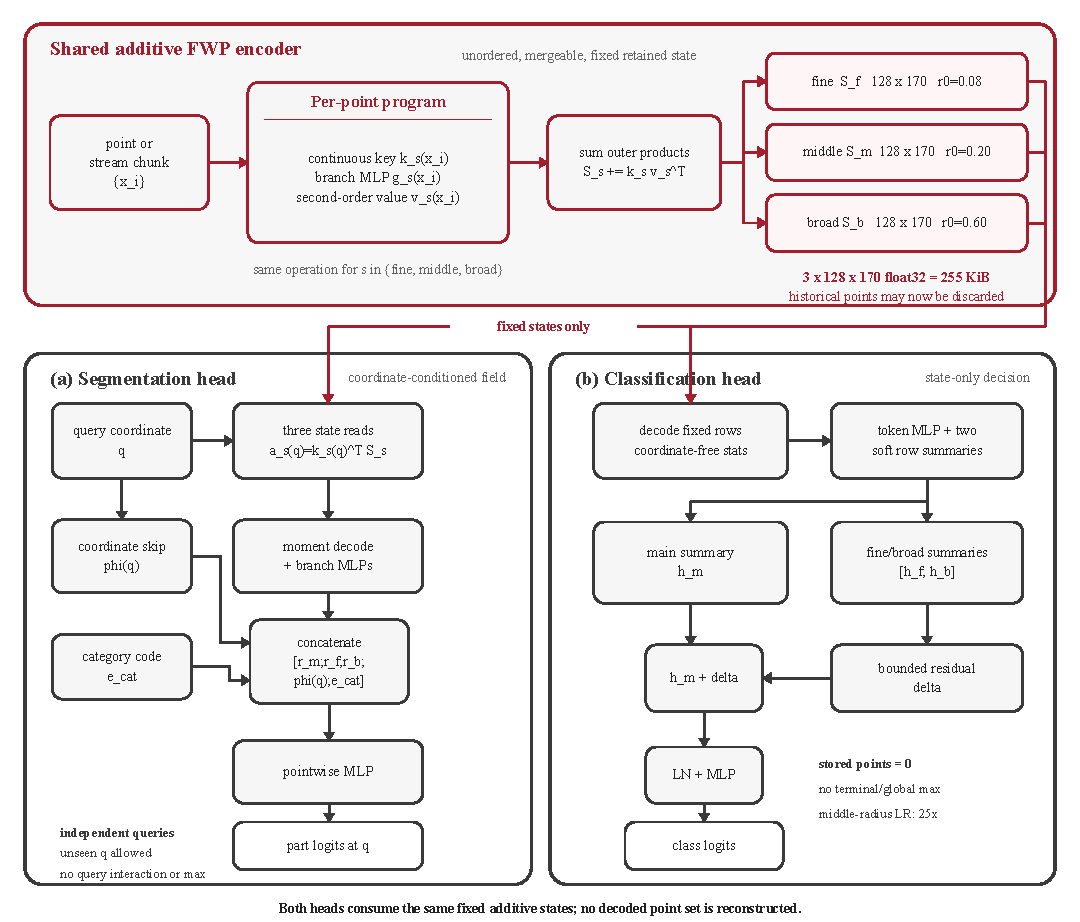
\includegraphics[width=\textwidth]{fig00_pointprogrammernet_architecture.pdf}
\caption{PointProgrammerNet 架构。历史点被删除后，红色路径传递三个等尺寸可加 FWP 状态。分割头在查询坐标 $\bm q$ 处读取每个状态，再拼接解码上下文、坐标跳连和类别编码。分类头解码固定状态行，并将有界的细尺度和粗尺度残差加到中尺度状态摘要上。两个任务头都不重建解码点集，也不对其执行池化。}
\label{fig:architecture}
\end{figure}

\subsection{将一个点写入状态}

每个分支的写入过程分别回答两个问题：当前点包含什么信息，以及这些信息应当写到矩阵的哪些行。

第一步，两层逐点网络把坐标变成 32 维特征：
\begin{equation}
\bm g_s(\bm x)=\operatorname{ReLU}\!\left(\operatorname{BN}\!\left(W_{s2}
\operatorname{ReLU}\!\left(\operatorname{BN}(W_{s1}\bm x+\bm b_{s1})\right)+\bm b_{s2}\right)\right)
\in\R^{32}.
\label{eq:content}
\end{equation}
其中，$s$ 是分支编号，$\bm x\in\R^3$ 是一个坐标，$W_{s1},W_{s2}$ 和 $\bm b_{s1},\bm b_{s2}$ 是可学习仿射参数，BN 表示 BatchNorm，$\bm g_s(\bm x)$ 是网络从该点提取的内容。两个隐藏仿射层宽度均为 32。三个分支使用各自独立的参数，因此状态尺寸相等并不会迫使它们学习相同特征。
这个非线性映射对每个点独立执行，因此它能增强单点写入的表达力，却不会让一个点的写入依赖其他点。持久状态仍然只累加随后形成的外积，所以这种逐点非线性不会破坏可加性。

第二步，用坐标决定当前点应写入 128 个状态行中的哪些位置。这里的 128 个“中心”不是从当前点云、训练集或某个物体中挑选的点，也不保存任何观测。它们是模型内部的 128 个可学习空间地址，每个状态行对应一个地址。训练开始前，Sobol 序列直接在 $[-0.9,0.9]^3$ 中生成 128 个分布较均匀的初始位置，使所有状态行一开始就覆盖整个归一化空间；三个分支各自获得一份可以独立学习的中心。训练时，$\bm c_{sj}=0.95\tanh(\bm\theta_{sj})$ 允许中心移动，同时保证它不会跑出坐标立方体。处理一个真实输入点 $\bm x$ 时，模型把它同时与全部 128 个中心比较，再把距离转换成 128 个连续写入比例。半径 $r_s=\exp(-\lambda_s)$ 决定这些比例是集中在少数邻近行，还是更均匀地分布到多行：
\begin{align}
\ell_{sj}(\bm x)&=-\frac{\|\bm x-\bm c_{sj}\|_2^2}{2r_s^2},\\
k_{sj}(\bm x)&=\frac{\exp \ell_{sj}(\bm x)}{\sum_{u=1}^{R}\exp \ell_{su}(\bm x)}.
\label{eq:key}
\end{align}
归一化使每个点的总写入质量恒为 1，因此半径只控制信息在状态行之间的集中程度，不会同时改变单个点的总幅值。每个点以连续权重写入所有行，距离较近的中心获得更大权重；这种设计避免最近中心硬选择造成的不连续边界，也不需要把当前点与其他输入点比较。较小半径形成更集中的局部统计，较大半径形成覆盖更广的统计。

可以把这 128 个中心理解成边界柔软、位置可学习的空间格子。一个输入点若靠近第 12 和第 47 个中心，这两行会得到较大比例，其余行只得到较小比例；模型不会把该点硬塞进某一行。这个 128 维地址只回答“写到哪里”，下一步构造的 170 维值则回答“写入什么”。二者外积后得到一次 $128\times170$ 更新：第 $j$ 行增加“第 $j$ 个写入比例乘以完整值向量”。所有点的更新相加后，每一行留下的是与该空间地址相关的一组累计统计，而不是原始点列表。

第三步，模型构造 170 维值向量：
\begin{equation}
\begin{aligned}
\bm v_s(\bm x)=[&1,\bm x,\bm g_s,\vect(\bm x\bm g_s^\top),\\
&x^2,y^2,z^2,xy,xz,yz,\bm g_s\odot\bm g_s].
\end{aligned}
\label{eq:value}
\end{equation}
各部分依次为 1 个单位质量、3 个坐标、32 个学习特征、96 个坐标与特征乘积、6 个几何二阶矩和 32 个特征平方项，总维度为 $1+3+32+96+6+32=170$。单位质量使累计和能够在读取时自行归一化；一阶项保存局部均值；坐标与特征乘积保存学习内容随位置变化的方式；两个二阶块保存均值会丢失的离散程度与相关关系。这些量都在逐点阶段计算，因此增加统计表达力不会破坏状态的可加性。

\begin{table}[htbp]
\centering
\caption{单个点写入的值向量。每个状态行都具有这 170 列。}
\begin{tabular}{lrl}
\toprule
组成 & 维度 & 保存的信息\\
\midrule
$1$ & 1 & 累计质量\\
$\bm x$ & 3 & 坐标和\\
$\bm g_s$ & 32 & 学习内容之和\\
$\bm x\bm g_s^\top$ & 96 & 位置与内容的关系\\
$\bm x\bm x^\top$ & 6 & 几何二阶矩\\
$\bm g_s\odot\bm g_s$ & 32 & 特征二阶矩\\
\bottomrule
\end{tabular}
\end{table}

一个点增加如下外积矩阵：
\begin{equation}
\Delta\Sstate_s(\bm x)=\bm k_s(\bm x)\bm v_s(\bm x)^\top,
\qquad
[\Delta\Sstate_s(\bm x)]_{j,:}=k_{sj}(\bm x)\bm v_s(\bm x)^\top.
\label{eq:single-write}
\end{equation}
该外积利用了 FWP 的关键特征：键选择状态行，值携带内容，各点的秩一写入直接相加。本文始终保留这种线性叠加，因此可加性直接来自 FWP，而非额外附加的技巧。矩阵行是连续加权累加器而非单点槽位，一批写入也可合并为一次矩阵乘法。对 $N$ 个点，令 $\bm K_s\in\R^{N\times128}$ 堆叠所有地址，$\bm V_s\in\R^{N\times170}$ 堆叠所有值，则
\begin{equation}
\Sstate_s(X)=\sum_{i=1}^{N}\bm k_s(\bm x_i)\bm v_s(\bm x_i)^\top
=\bm K_s^\top\bm V_s\in\R^{128\times170}.
\label{eq:state}
\end{equation}
其中，$i$ 是输入点编号，$j$ 是固定状态行编号。在流式处理中，模型只为新到达的分块计算 $\bm K_s^\top\bm V_s$，将结果加到持久状态后即可释放该分块。除浮点累加顺序造成的微小误差外，如何划分分块不会改变最终状态。

完整的流式流程只有四步：首先在共享参考坐标系中归一化新分块；其次为三个分支计算地址矩阵和值矩阵；然后把三个 $\bm K_s^\top\bm V_s$ 加到持久状态；最后释放全部与该分块有关的临时张量。分布式设备执行相同操作，只发送三个固定矩阵。推理时，分割头只计算感兴趣的查询坐标，分类头则直接使用状态矩阵。任何后续阶段都不需要从状态中重新生成点列表。

\subsection{分割读出}

分割任务需要预测坐标 $\bm q\in\R^3$ 处的部件类别。这里，$\bm x_i$ 是已经写入状态的观测点，写入后可以从内存中删除；$\bm q$ 只是需要预测标签的位置。ShapeNetPart 在有标签的原始点坐标上评估，因此实验中通常令查询坐标等于某个原始点坐标，但解码器只接收该坐标和固定状态，并不重新读取这个点的原始特征。模型用写入时相同的中心和半径计算 $\bm k_s(\bm q)$，再从状态行中读取加权组合：
\begin{equation}
\bm a_s(\bm q)=\bm k_s(\bm q)^\top\Sstate_s
=\sum_i w_{si}(\bm q)\bm v_s(\bm x_i)^\top,
\quad
w_{si}(\bm q)=\bm k_s(\bm q)^\top\bm k_s(\bm x_i).
\label{eq:effective-weight}
\end{equation}
其中，$\bm a_s(\bm q)\in\R^{170}$ 是原始读取结果。$w_{si}(\bm q)$ 只是把矩阵乘法展开成逐点形式后的解释：如果观测点 $i$ 写入较多的状态行也正是查询坐标 $\bm q$ 重点读取的状态行，这个系数就较大。实际推理不会逐点计算 $w_{si}$，而是直接计算 $\bm k_s(\bm q)^\top\Sstate_s$；它不还原或遍历历史点，也不对解码后的点特征执行全局最大值汇聚。

令 $\mu_s(\bm q)=\sum_iw_{si}(\bm q)$ 表示读取质量。为防止分母接近零，实现中使用
\begin{equation}
\epsilon_s=10^{-3}\operatorname{mean}_{\bm q'}\mu_s(\bm q')+10^{-20},
\qquad
\widetilde\mu_s(\bm q)=\max(\mu_s(\bm q),\epsilon_s),
\end{equation}
其中，$\bm q'$ 遍历同一样本的查询坐标。这个停止梯度的数值下限只使用查询质量，不汇集点特征，也不会在查询之间传播梯度；单个坐标仍可独立计算。为简化记号，令 $w_i=w_{si}(\bm q)$，则状态中保存的各类和可以还原为
\begin{align}
\bar{\bm x}_s&=\widetilde\mu_s^{-1}\sum_iw_i\bm x_i,&
\bar{\bm g}_s&=\widetilde\mu_s^{-1}\sum_iw_i\bm g_s(\bm x_i),\nonumber\\
E_{xg,s}&=\widetilde\mu_s^{-1}\sum_iw_i\bm x_i\bm g_s(\bm x_i)^\top,&
E_{xx,s}&=\widetilde\mu_s^{-1}\sum_iw_i\bm x_i\bm x_i^\top,\nonumber\\
E_{gg,s}&=\widetilde\mu_s^{-1}\sum_iw_i\bm g_s(\bm x_i)\odot\bm g_s(\bm x_i).&&
\label{eq:read-moments}
\end{align}
其中，$\bar{\bm x}_s$ 和 $\bar{\bm g}_s$ 是局部坐标均值与特征均值；$E_{xg,s}$ 描述位置和学习内容如何共同变化；$E_{xx,s}$ 描述几何分布；$E_{gg,s}$ 描述特征能量。这些量都来自一次矩阵读取。

模型把上述量整理成
\begin{equation}
\begin{aligned}
\bm d_s(\bm q)=[&\bar{\bm g}_s,\bar{\bm x}_s-\bm q,\log\widetilde\mu_s,
\vect(E_{xg,s}-\bm q\bar{\bm g}_s^{\top}),\\
&\operatorname{vech}(E_{xx,s}-\bar{\bm x}_s\bar{\bm x}_s^{\top}),
\sqrt{[E_{gg,s}-\bar{\bm g}_s\odot\bar{\bm g}_s]_++10^{-8}}].
\end{aligned}
\label{eq:query-decode}
\end{equation}
其中，$\operatorname{vech}$ 保留对称 $3\times3$ 矩阵的 6 个互异元素，$[\cdot]_+$ 将浮点误差造成的微小负方差截断为零。六个部分的维度分别为 $32,3,1,96,6,32$，依次表达局部内容、局部中心相对查询的位移、可用证据量、位置与内容的关系、几何协方差和特征标准差。

三个分支都独立使用完全相同的 $170\rightarrow160\rightarrow160$ 网络，并在每层后使用 BatchNorm 和 ReLU，最终得到 $\bm r_s(\bm q)\in\R^{160}$。任何分支都没有更宽或更深的解码器。三个结果直接拼接，使最终网络可以分别利用不同初始空间范围的信息：
\begin{equation}
\bm z_{\rm seg}(\bm q)=h_{\rm seg}([\bm r_f;\bm r_m;\bm r_b;\phi(\bm q);\bm e_{\rm cat}]).
\label{eq:seg}
\end{equation}
三个分支的解码结果保持分离，使最终网络可以比较不同学习空间范围的证据，而不会在读取后立即平均。$\phi(\bm q)\in\R^{32}$ 保留精确查询位置，$\bm e_{\rm cat}\in\R^{16}$ 则利用物体类别限制合理的部件标签。$h_{\rm seg}$ 的尺寸为 $528\rightarrow256\rightarrow128\rightarrow50$，前两个仿射层后使用 BatchNorm、ReLU 和 0.3 dropout。坐标路径相当于绕过状态压缩的 U-Net 式跳连：历史上下文必须经过三个固定矩阵，查询点身份则保持精确。分割头不对查询点执行最大池化，也不在查询点之间交换学习特征，因此历史点特征可以删除；同一状态还可查询原点集中不存在的坐标，但本文尚未测量这种插值能力。

\subsection{分类读出}

分类任务没有查询坐标，也不保留输入点。模型先把固定状态的每一行还原为归一化统计量。把 $\Sstate_s$ 的第 $j$ 行写成
\begin{equation}
[\mu_{sj},\bm p_{sj},\bm f_{sj},\vect(\bm C_{sj}),\operatorname{vech}(\bm Q_{sj}),\bm u_{sj}],
\label{eq:row-sums}
\end{equation}
其中，$\mu_{sj}\in\R$ 是累计质量，$\bm p_{sj}\in\R^3$ 是坐标和，$\bm f_{sj}\in\R^{32}$ 是特征和，$\bm C_{sj}\in\R^{3\times32}$ 是坐标与特征乘积的和，$\bm Q_{sj}\in\R^{3\times3}$ 是对称的坐标二阶矩之和，$\bm u_{sj}\in\R^{32}$ 是特征平方和。$\bm Q_{sj}$ 只需保存六个互异元素。为防止分母接近零，定义
\begin{equation}
\widetilde\mu_{sj}=\max\!\left(\mu_{sj},10^{-4}R^{-1}\sum_{u=1}^{R}|\mu_{su}|+10^{-20}\right).
\end{equation}
数值下限随当前状态的平均质量自适应，并在反向传播时视为常数。这样既能阻止近空状态行产生不稳定比值，也不会对总质量不同的物体强加同一个绝对阈值。再令 $\bar\mu_s=R^{-1}\sum_u\widetilde\mu_{su}$、$\bar{\bm x}_{sj}=\bm p_{sj}/\widetilde\mu_{sj}$、$\bar{\bm g}_{sj}=\bm f_{sj}/\widetilde\mu_{sj}$、$E_{xg,sj}=\bm C_{sj}/\widetilde\mu_{sj}$、$E_{xx,sj}=\bm Q_{sj}/\widetilde\mu_{sj}$、$E_{gg,sj}=\bm u_{sj}/\widetilde\mu_{sj}$。送入行网络的向量为
\begin{equation}
\begin{aligned}
\bm d^{\rm row}_{sj}=[&\bar{\bm g}_{sj},\bar{\bm x}_{sj},
\log(\widetilde\mu_{sj}/\bar\mu_s),
\operatorname{vech}(E_{xx,sj}-\bar{\bm x}_{sj}\bar{\bm x}_{sj}^{\top}),\\
&\sqrt{[E_{gg,sj}-\bar{\bm g}_{sj}\odot\bar{\bm g}_{sj}]_++10^{-8}},
\vect(E_{xg,sj}-\bar{\bm x}_{sj}\bar{\bm g}_{sj}^{\top})].
\end{aligned}
\label{eq:row-descriptor}
\end{equation}
六个部分的维度依次为 $32,3,1,6,32,96$，合计 170。它们分别表示特征均值、质心、相对行质量、坐标协方差、特征标准差以及坐标与特征的协方差。这与分割读出的统计量相对应；除以 $\widetilde\mu_{sj}$ 后，累计和变成均值，使不同输入点数得到的量处于可比较的尺度。

每个分支使用独立的 $170\rightarrow128\rightarrow128$ 行编码网络，并使用 LayerNorm 和 GELU。令 $\bm T_s\in\R^{R\times128}$ 表示编码后的 128 行。随后，两组可学习评分分别对这 128 行做加权求和：
\begin{equation}
\begin{aligned}
\bm U_s&=\operatorname{softmax}_{\rm rows}(\operatorname{score}_s(\bm T_s))
\in\R^{R\times2},\\
\bm h_s&=H_s\!\left(\vect(\bm U_s^\top\bm T_s)\right)\in\R^{256}.
\end{aligned}
\label{eq:state-summary}
\end{equation}
其中，$\operatorname{score}_s:\R^{128}\rightarrow\R^2$ 为每一行产生两个分数；softmax 分别在两列分数的 128 行上归一化；$\bm U_s$ 保存两组行权重；$H_s:\R^{256}\rightarrow\R^{256}$ 由仿射层、LayerNorm 和 GELU 组成；$\bm h_s$ 是分支摘要。这里汇总的是固定 128 行矩阵，而不是长度随输入变化的点列表，因此存储量和读出开销不随历史点数增长。

中尺度摘要作为参考，细尺度和粗尺度摘要提供有界修正：
\begin{align}
\bm\delta&=\sigma(a)\tanh(W[\bm h_f;\bm h_b]+\bm b),\\
\bm z_{\rm cls}&=h_{\rm cls}(\operatorname{LN}(\bm h_m+\bm\delta)).
\label{eq:cls}
\end{align}
投影把细、粗摘要映射到中尺度摘要的 256 维空间，$\sigma(a)\tanh(\cdot)$ 则限制辅助分支能够改变参考表示的幅度。受控实验发现，纯状态分类器采用直接拼接时更难优化，因此这里保留以中尺度为稳定路径的有界修正。分类器 $h_{\rm cls}$ 为 $256\rightarrow256\rightarrow40$，使用 GELU 和 0.3 dropout。残差投影从零开始，$\sigma(a)$ 初始为 0.1，使训练先获得可用的中尺度表示，再逐渐接纳细、粗尺度证据。三个半径均可学习；中尺度半径使用 $25\times$ 学习率且不使用权重衰减，其余参数使用基础优化器设置。

\subsection{形式性质}

\begin{proposition}[置换不变性与可加性]
对每个分支，式~\eqref{eq:state} 与点的输入顺序无关，并且
$\Sstate_s(\biguplus_tX_t)=\sum_t\Sstate_s(X_t)$。
\end{proposition}
其中，$t$ 是任意点分块的编号，$X_t$ 是第 $t$ 个分块。
\begin{proof}
每个点只贡献一个矩阵。有限和在实数运算中与加法顺序和分组无关；实际计算中的微小差异仅来自浮点累加顺序。
\end{proof}

\begin{corollary}
分块可直接相加。若已保存子集状态 $\Sstate_s(Y)$，则
$\Sstate_s(X\setminus Y)=\Sstate_s(X)-\Sstate_s(Y)$。指数遗忘为
$\Sstate_{s,t}=\rho\Sstate_{s,t-1}+\Sstate_s(X_t)$，其中 $0\le\rho\le1$。
\end{corollary}
其中，$Y$ 是需要删除的点子集，$t$ 是帧编号，$X_t$ 是新到达的帧，$\rho$ 是上一时刻状态的保留比例。

\begin{corollary}[分布式等价性]
设设备 $d$ 在共享坐标系中观察到多重集合 $X^{(d)}$，并使用相同编码器。中心节点可以构造
\begin{equation}
\Sstate_s^{\rm global}=\sum_{d=1}^{D}\Sstate_s(X^{(d)})
=\Sstate_s\!\left(\biguplus_{d=1}^{D}X^{(d)}\right).
\label{eq:distributed}
\end{equation}
因此，无论使用哪一种任务头，其输入状态都与集中式编码相同，差别只可能来自浮点累加顺序。
\end{corollary}
其中，$D$ 是设备数量，$d$ 是设备编号，$X^{(d)}$ 是设备 $d$ 的本地点多重集合，$\Sstate_s^{\rm global}$ 是中心节点得到的分支状态。

式~\eqref{eq:distributed} 将感知与推理解耦。设备可在编码后删除本地点，只发送三个固定矩阵；中间节点也可按任意树结构或到达顺序继续求和。服务器执行分类只需合并状态；执行分割还需要待查询坐标及类别编码。严格等价要求所有设备共享模型权重、坐标归一化方式和参考坐标系。

\begin{proposition}[固定存储和增量更新]
保留内存为 $O(\sum_sR_sD_s)$，与历史点数无关。编码 $M$ 个新点的外积开销为 $O(M\sum_sR_sD_s)$，也与历史长度无关。
\end{proposition}
其中，$R_s$ 和 $D_s$ 分别是分支 $s$ 的行数和列数，$M$ 是新到达的点数。
\begin{proof}
系统只保留固定矩阵；无论先前包含多少分块，新分块都产生同样规模的矩阵乘法。
\end{proof}

\begin{proposition}[证据和查询的连续性]
对证据强度 $t\in[0,1]$，令
\begin{equation}
\Sstate_s(t)=\Sstate_s^{\rm old}+t\,\bm k_s(\bm x)\bm v_s(\bm x)^\top.
\label{eq:path}
\end{equation}
分类 logits 和固定查询坐标下的分割 logits 对 $t$ 连续且分段光滑；固定状态下的分割 logits 对 $\bm q$ 连续且分段光滑。
\end{proposition}
其中，$\Sstate_s^{\rm old}$ 是写入新观测前的状态，$\bm x$ 是该观测，$t$ 将其证据强度从未写入（$t=0$）调节到完整写入（$t=1$）。
\begin{proof}
状态是 $t$ 的仿射函数。式~\eqref{eq:key} 中的高斯距离权重、softmax、线性层、使用正数下限的除法、ReLU/GELU 和加入稳定常数的平方根都是连续函数；它们的复合也是连续且分段可微的。
\end{proof}
状态随证据强度线性变化。Logits 和概率通常以非线性但连续的方式变化；离散的 argmax 标签则可在决策边界处跳变。该连续性来自模型方程；校准和时间稳定性仍需通过实验回答。

\subsection{未来的帧级 delta 规则}

令 $\bm K_{s,t},\bm V_{s,t}$ 打包第 $t$ 帧的全部点，未来可研究以下自适应状态转移：
\begin{equation}
\Sstate_{s,t}=\rho\Sstate_{s,t-1}+\eta_t\bm K_{s,t}^{\top}
(\bm V_{s,t}-\bm K_{s,t}\Sstate_{s,t-1}).
\label{eq:delta}
\end{equation}
其中，$\bm K_{s,t}$ 和 $\bm V_{s,t}$ 分别包含第 $t$ 帧在分支 $s$ 上的全部键和值，$\rho$ 是旧状态保留比例，$\eta_t$ 是 delta 更新步长。
该形式来自快速权重 delta 规则~\cite{schlag2021linear}。若帧内点顺序由置换矩阵 $P$ 改变，则 $\bm K'=P\bm K$、$\bm V'=P\bm V$；由于 $P^\top P=I$，修正项保持不变。因此帧内点仍是无序的，而帧顺序进入递归状态。该扩展会主动放弃跨帧的严格可加性，本文实验未使用它。

\section{实验}

\subsection{实验协议}

每个物体先中心化，再用 XYZ 最大绝对坐标归一化；每个样本使用 1,024 个点。ShapeNetPart 包含 13,972 个训练形状和 2,874 个测试形状；ModelNet40 包含 9,840 个训练形状和 2,468 个测试形状。模型训练 20 个 epoch，使用 AdamW、基础学习率 $3\times10^{-3}$、权重衰减 $10^{-4}$ 和余弦衰减；分割和分类批大小分别为 16 和 32。分类使用 0.1 标签平滑。所有结果报告种子 0、1、2 的均值和总体标准差。密度偏移测试按 $\exp(2.5\bm x^\top\bm d)$ 给点分配无放回采样概率，其中 $\bm d$ 是由固定随机种子生成的单位方向。紧凑 PointNet++ 是本地受控基线。分类实验中的较宽 PointNet 有 442,838 个参数，与 529,426 参数的纯状态分类模型并非严格配平。

\subsection{准确率}

\begin{table}[htbp]
\centering
\caption{ShapeNetPart 部件分割结果。输入为 XYZ，每个样本 1,024 个点，结果为三个随机种子的均值 $\pm$ 总体标准差。}
\resizebox{\textwidth}{!}{%
\begin{tabular}{lrrrr}
\toprule
模型 & 点准确率 & 实例 mIoU & 类别 mIoU & 参数量\\
\midrule
轻量 PointNet++ & $93.41\pm0.05$ & $83.88\pm0.11$ & $79.51\pm0.24$ & 573,106\\
PointProgrammerNet & $92.95\pm0.02$ & $82.58\pm0.15$ & $79.10\pm0.25$ & 341,909\\
\bottomrule
\end{tabular}
}
\end{table}

PointProgrammerNet 的点准确率、实例 mIoU 和类别 mIoU 分别比轻量 PointNet++ 低 0.46、1.30 和 0.41 个百分点，但参数量少 40.3\%，并且不对历史点或解码后的查询点执行最大池化。

\begin{table}[htbp]
\centering
\caption{ModelNet40 分类结果。结果为三个随机种子的均值 $\pm$ 总体标准差。}
\resizebox{\textwidth}{!}{%
\begin{tabular}{lrrrr}
\toprule
模型 & 干净准确率 & 密度偏移准确率 & 下降 & 参数量\\
\midrule
轻量 PointNet++ & $89.84\pm0.43$ & $85.47\pm0.88$ & $4.38\pm1.18$ & 207,784\\
较宽 PointNet & $87.90\pm0.27$ & $87.55\pm0.38$ & $0.35\pm0.12$ & 442,838\\
PointProgrammerNet & $86.59\pm0.23$ & $82.47\pm0.93$ & $4.12\pm0.71$ & 529,426\\
\bottomrule
\end{tabular}
}
\end{table}

纯状态分类器达到 $86.59\%$ 干净准确率，比轻量 PointNet++ 低 3.25 个百分点，比较宽 PointNet 低 1.31 个百分点。密度偏移下准确率下降 4.12 个百分点。因此，分类可以仅从可合并状态完成而不保留输入点，其代价是可测量的精度下降。

\subsection{可加性与固定状态}

\begin{figure}[htbp]
\centering
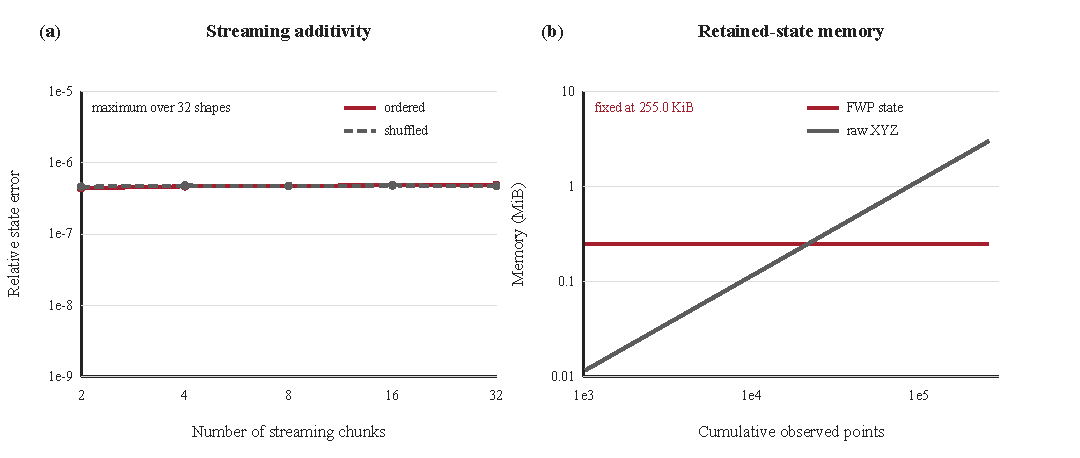
\includegraphics[width=.98\textwidth]{fig01_additivity_fixed_state.pdf}
\caption{可加流式处理与固定保留内存。有序和乱序分块写入都能在浮点累加误差范围内复现单批次 FWP 状态。无论点流多长，三个 $128\times170$ 的 float32 状态始终占用 255 KiB；保存 XYZ 坐标所需的内存则随观测数量线性增长。}
\label{fig:additivity_fixed_state}
\end{figure}

在 32 个物体上，将点云分成 2 至 32 个有序或乱序分块后构造状态；所得结果与一次性构造的最大相对误差低于 $5.3\times10^{-7}$。这也模拟了多个设备分别编码互不重叠的点子集，再由服务器相加。三个状态共含 65,280 个 float32 标量，即 255 KiB。固定内存不意味着任何情况下都更省内存：裸 XYZ 要到 21,760 点才达到 255 KiB，而 1,024 点的 XYZ 点云明显更小。优势在于点流持续增长时，保留内存仍有严格上界，而且状态保存的是学习得到的几何统计量，而非仅保存原始坐标。

\subsection{状态操作}

\begin{figure}[htbp]
\centering
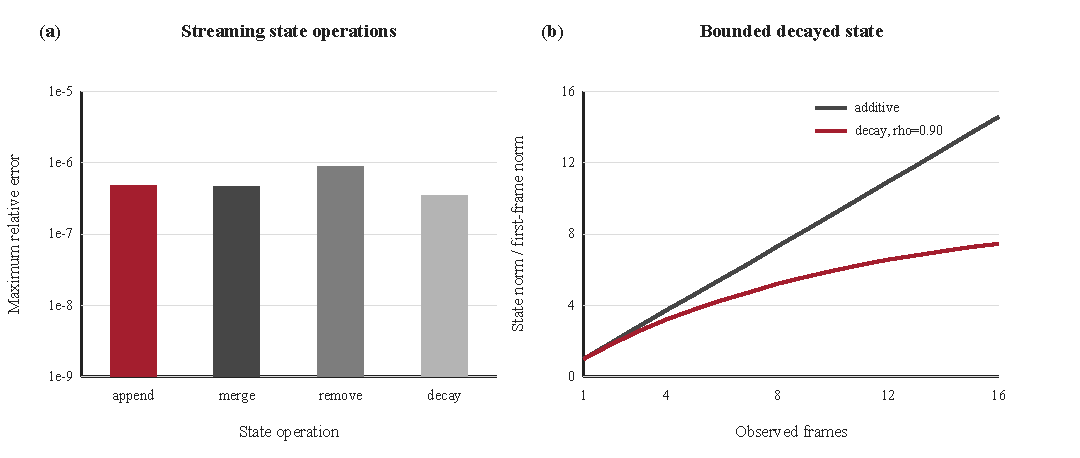
\includegraphics[width=.98\textwidth]{fig02_state_operations.pdf}
\caption{流式状态操作。（a）追加或合并、帧删除和指数衰减相对于独立重建 FWP 状态的最大相对误差，测试对象为 32 个 ShapeNetPart 物体。（b）普通加法使状态幅值随帧数增长；指数衰减在不改变状态尺寸的情况下限制旧帧的影响。}
\label{fig:streaming-state-operations}
\end{figure}

追加、合并、删除和指数衰减相对于独立重建的平均相对误差分别为 $2.11\times10^{-7}$、$2.13\times10^{-7}$、$3.03\times10^{-7}$ 和 $1.77\times10^{-7}$，最大值都低于 $9.8\times10^{-7}$。经过 16 帧，普通加法状态范数为 14.51；使用 $\rho=.9$ 的衰减后，范数限制在 7.42。此实验验证状态代数，不代表时序任务准确率。

\subsection{流式效率}

\begin{figure}[htbp]
\centering
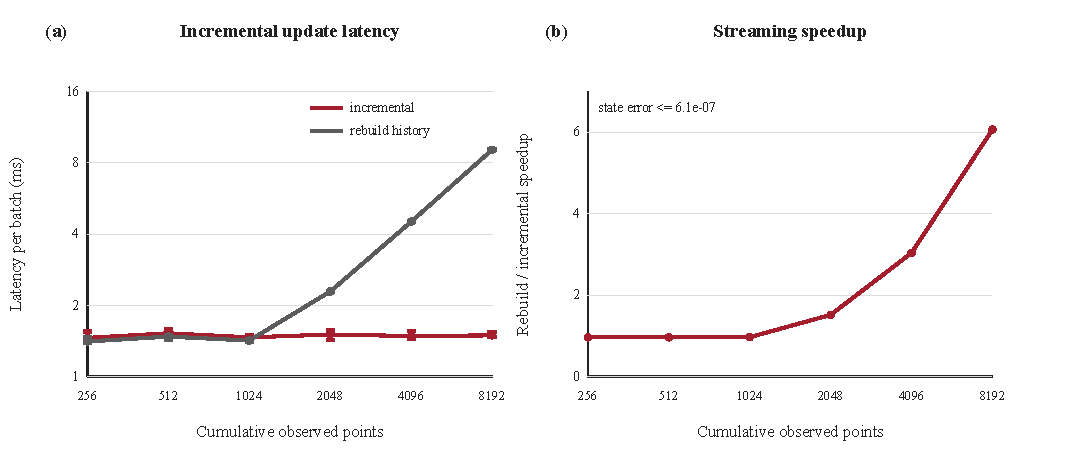
\includegraphics[width=.98\textwidth]{fig04_streaming_efficiency.pdf}
\caption{设备内存常驻点流的 FWP 状态构建开销。（a）增量更新只处理新增的 256 点帧，而重建会处理所有累计点。数据为四条点流、每次 30 次重复、七轮交错试验的挂钟时间中位数，误差线表示观测范围。（b）速度提升随历史长度增加，同时增量状态与重建状态保持数值等价。}
\label{fig:streaming-efficiency}
\end{figure}

在 RTX 3070 Ti Laptop GPU 上，我们对四条常驻设备内存的点流计时，每帧加入 256 个点；每个设置重复 30 次并进行七轮试验。增量更新延迟稳定在约 1.46--1.53 ms。由于启动固定尺寸更新本身存在开销，在累计点数不超过 1,024 时重建略快；到 2,048、4,096 和 8,192 点时，增量更新分别快 $1.52\times$、$3.04\times$ 和 $6.06\times$。状态相对误差始终低于 $6.1\times10^{-7}$。

\subsection{受控架构审查}

\begin{figure}[htbp]
\centering
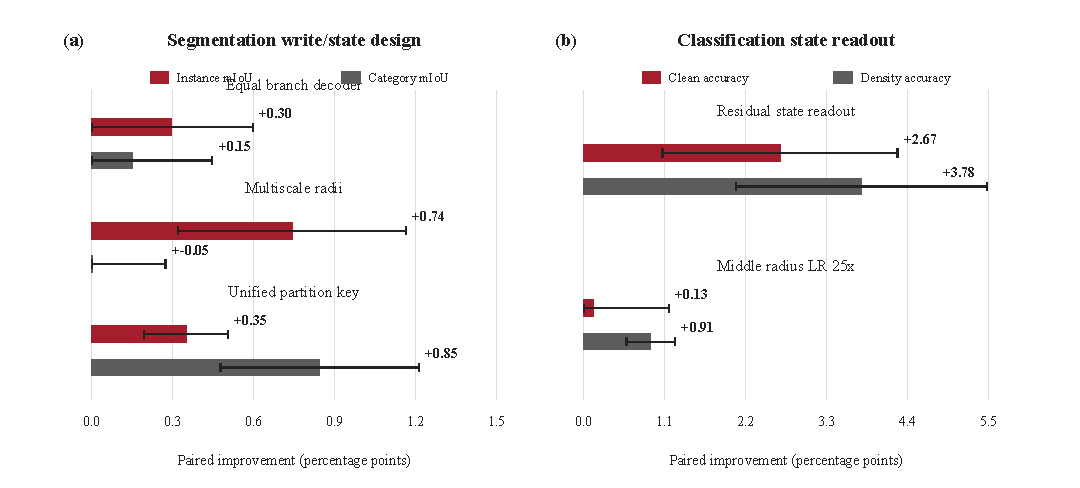
\includegraphics[width=.98\textwidth]{fig03_controlled_ablation.pdf}
\caption{三个随机种子的筛选消融实验。分割部分将最终模型分别与不等分支解码器、相同初始半径和混合空间地址公式进行比较；纯状态分类部分比较中尺度参考残差与直接拼接，并改变中尺度半径学习率。柱高表示配对均值变化，误差线表示总体标准差。每次筛选训练五个 epoch。}
\label{fig:architecture_ablation}
\end{figure}

五轮、三种子的快速实验每次只改变一个选择。三个分割分支都采用 $170\rightarrow160\rightarrow160$ 解码器后，实例 mIoU 变化为 $+0.30\pm0.30$ 个百分点，类别 mIoU 变化为 $+0.15\pm0.29$，同时减少 24,480 个参数。使用不同的初始半径使实例 mIoU 提高 $0.74\pm0.42$，类别 mIoU 基本不变（$-0.05\pm0.33$）。三个分支统一使用式~\eqref{eq:key} 的归一化空间地址后，相比混合地址公式，实例和类别 mIoU 分别提高 $0.35\pm0.16$ 和 $0.85\pm0.37$。分类中，以中尺度为参考的残差相比直接拼接，使干净准确率和密度偏移准确率分别提高 $2.67\pm1.60$ 和 $3.78\pm1.71$。中尺度半径使用 $25\times$ 学习率后，干净准确率变化不稳定（$0.13\pm1.03$），但偏移准确率稳定提高（$0.91\pm0.33$），因此保留这一设置以改善鲁棒性。

\section{讨论与局限}

本方法面向持续增长或分布式产生的点流。单个传感器可以编码一帧、合并状态并释放该帧。多个相机、LiDAR、机器人或边缘处理器可以分别编码不同空间区域或时间窗，再将固定状态发送给服务器。矩阵加法给出与集中式编码相同的表示，因此允许异步到达和分层聚合，原始点集无需离开感知设备。分割服务只需保留计划查询的坐标，分类器则可在不重放历史点的情况下更新证据。这些操作都不需要把新点与全部历史解码点比较。

\subsection{分布式推理示例}

考虑多个 LiDAR 节点观察同一场景的不同部分。训练完成的编码器复制到每个节点，所有节点使用相同的归一化方式，并把坐标表达在公共参考系中。节点 $d$ 把本地点分块编码成 $\{\Sstate_f^{(d)},\Sstate_m^{(d)},\Sstate_b^{(d)}\}$，随后即可删除本地点特征。中继节点可以任意合并这些状态，服务器最终执行式~\eqref{eq:distributed}。无论状态以什么顺序到达，或者通信采用怎样的树形结构，实数运算下的结果都相同。每个节点发送的三个矩阵始终为 255 KiB，与本地分块包含几百个点还是代表长期累计点流无关。

分类时，服务器直接把合并后的三个矩阵送入状态行读出。增加一个设备或一帧数据，只需再加一组三矩阵，不必重新解码和汇总旧点云。分割时，服务器把坐标 $\bm q$ 送入三个矩阵读取。查询坐标可以是选定的观测点、操作人员关心的区域，也可以是规则网格上的位置。读取阶段只需保留这些坐标。由于式~\eqref{eq:effective-weight} 对 $\bm q$ 连续，附近位置得到的状态证据也会平滑变化，包括原点集中没有直接观测的位置。当前实验只评估 ShapeNetPart 的已观测点，因此对新坐标的插值准确率仍需另行验证。

固定状态是摘要，不是用于还原原始点的压缩档案。它足以计算已经训练好的任务头，但并不保证重建每个观测。当大量空间地址相互重叠时，不同点集可能产生相近的矩统计量。学习中心、半径、内容网络和二阶项共同决定哪些差异能在压缩后保留下来。这同时解释了固定内存的优势，以及模型相比分层邻域方法仍存在的精度差距。

固定状态同时也是信息瓶颈。PointNet++ 会围绕真实观测点构造邻域，PointNet 会保留逐通道极值；PointProgrammerNet 只保留有限个学习矩表。这可以解释其离线精度差距，分类任务尤其明显。对小点云而言，固定状态也可能比裸 XYZ 更占内存；每个设备都发送一个状态，只有当系统需要固定通信上界或面对长时间点流时才有明显价值。分布式严格等价还要求公共坐标系和一致预处理。分割仍需对每个查询坐标执行一次状态读取。

法线、颜色或强度可以加入值通道，同时继续用 XYZ 建立空间键；法线也可以参与乘积键，但需要处理方向和带宽。当前实验每个任务只覆盖一个数据集，使用 XYZ 输入，只在一块 GPU 上计时，并采用本地受控基线。本文尚未测量不存在坐标的查询精度、时序校准、逐点类别稳定性或 delta 自适应。连续 logits 不意味着预测一定单调改善，也不保证离散标签连续。

\section{结论}

PointProgrammerNet 用固定可加矩阵概括点云。连续键和二阶值支持无序写入、精确分布式合并、删除、衰减，以及与历史长度无关的增量更新。坐标条件分割和纯状态分类都不在解码点之间做池化。虽然准确率仍低于分层基线，但该模型为集中式或分布式点云推理提供了一个紧凑、可检验、存储有界的流式设计。

\section*{CRediT 作者贡献声明}

Dian Yu：概念提出、方法设计、软件实现、验证、形式分析、实验、数据整理、可视化、初稿撰写及修改。

\section*{数据可得性}

复现论文所报告模型所需的代码作为补充材料提供。ShapeNetPart 和 ModelNet40 均为公开数据集，可从本文引用的原始来源获得。

\bibliographystyle{plain}
\bibliography{../manuscript/references}
\end{document}


